\documentclass{beamer}

\usepackage{wrapfig}
\usepackage{algpseudocode}
\usepackage{algorithm}
\usepackage[export]{adjustbox}
\usepackage{svg}

\usetheme{Boadilla}
\usecolortheme{dolphin}
\setbeamertemplate{navigation symbols}{}
\setbeamertemplate{sections/subsections in toc}[sections numbered]

\setbeameroption{hide notes}
% \setbeameroption{show only notes}
% \setbeameroption{show notes on second screen=right}

\title[Adaptive Embedded Trace]
{Adaptive Embedded Trace: Assessment of Ideas}
\author[]{Hossein Afkar}
\institute{DRTS Lab}
\date{\today}

\begin{document}

\frame{\titlepage}

\begin{frame}
    \frametitle{Outline}
    \tableofcontents[hideallsubsections]
\end{frame}

\AtBeginSection[]
{
    \begin{frame}{Outline}
        \tableofcontents[currentsection]
    \end{frame}
}

\section{Preface}
\begin{frame}
    \frametitle{Preface}
    \begin{itemize}
        \item Embedded Trace in Cyber-Physical Systems.
        \item Exploring Fault Detection.
        \item Memory Bandwidth control.
    \end{itemize}
\end{frame}

\section{Embedded Trace in Cyber-Physical Systems}
\begin{frame}
    \frametitle{Introduction}
    \begin{itemize}
        \item Advanced embedded system technology is one of the key
            driving forces behind the rapid growth
            of Cyber-Physical System (CPS) applications.
        \item Advanced architectures create challenges for testing and
            verification.
            \begin{itemize}
                \item Observability.
                \item Non-intrusiveness
            \end{itemize}
        \item A promising technology to address the observability issue is
            Embedded Trace (ET).
            \begin{itemize}
                \item Opens the window to the systems behaviour while
                    executing software.
                    \begin{itemize}
                        \item Revealing memory access patterns
                        \item Execution control
                        \item Data flow
                        \item Protocol sequences
                    \end{itemize}
            \end{itemize}
    \end{itemize}
\end{frame}

\begin{frame}
    \frametitle{Noted Excerpts From The Paper}
    \begin{itemize}
        \item Data-Flow messages are large and can consume trace bandwidth.
        \item ETM evolution:
            \begin{itemize}
                \item ETMv1 and ETMv2 report the pipeline state in a cycle by
                    cycle basis.
                \item ETMv3 abolishes pipeline state and introduces P-Header
                    packets that represent the state of the instructions.
                \item ETMv3 to ETMv1 only output the information of the flow of
                    execution when it can not be inferred from the execution
                    image.
                \item Observeability tradeoffs can be solved using ITM.
                \item ETMv4 reports the cancellation or completion of
                    speculative code execution.
            \end{itemize}
    \end{itemize}
\end{frame}
\section{Fault Detection and Adaptation}
\begin{frame}
    \frametitle{Exploring What It Means to Adapt}
    \begin{itemize}
        \item Adaptability is defined in relation to a feature.
        \item Fault detection and various online error detection methods come
            to mind when mentioning adaptability.
        \item In order to be adaptable we should define what we need to adapt
            for
            \begin{itemize}
                \item Adapt to ?
            \end{itemize}
    \end{itemize}
\end{frame}
\begin{frame}
    \frametitle{Online Error Detection Through Trace Infrastructure in
    ARM Microprocessors}
    \begin{itemize}
        \item there is a growing interest in the use of COTS microprocessors
            in space applications.
        \item Particularly for small satellites with tight budget constraints
            and missions that require high processing power.
        \item Experimental results demonstrate high accuracy with up to 95\% 
            of observed errors detected in a commercial microprocessor with
            no hardware modification using ETM and ITM.
    \end{itemize}
\end{frame}
\begin{frame}
    \frametitle{Hardware Accelerated Trace Analysis for Compiler Optimizations}
    \begin{itemize}
        \item Master thesis from the ETH Zurich
        \item Works on Profile Guided Optimizations present in compilers.
        \item Uses ETMv4 for trace collection.
        \item Proposes FPGA based trace collection.
            \begin{itemize}
                \item Increased data collection reliablity
                \item Increased Throughput.
                \item On-Chip data processing.
            \end{itemize}
    \end{itemize}
\end{frame}
\begin{frame}
    \frametitle{Categorizing Fault in Embededd Systems}
    \begin{itemize}
        \item Timing Faults
        \item Power
    \end{itemize}
\end{frame}
\section{Temporal Independece for Memory Subsystem}
\begin{frame}
    \frametitle{Temportal Independece for Memory Subsystems}
    \begin{itemize}
        \item Convectional memory controllers are not designed to handle
            mixed-criticality software.
        \item In these cases WCET is defined for all possible memory
            transcations which is far tighter than the normal case of the
            single-core processors.
        \item Different strategies are used such as:
            \begin{itemize}
                \item Designing custom real-time controllers.
                \item Software based strategies using interrupts like MemGuard.
                \item Transactional Memory.
            \end{itemize}
    \end{itemize}
\end{frame}
\begin{frame}
    \frametitle{MemGuard: Memory Bandwidth Reservation System for Efficient
    Performance Isolation in Multi-core Platforms}
    \begin{itemize}
        \item Memory bandwidth in modern multi-core platforms is highly
            variable
        \item And it is a big challenge in designing real-time systems as
            applications are becoming increasingly more memory intensive.
        \item MemGuard:
            \begin{itemize}
                \item Reserve memory for every core to achieve temporal
                    correctness.
                \item Reclaim unused bandwidth to maximize performance.
                \item Divides bandwidth to guranteeed and best-effort.
                \item Mainly target soft real-time systems
                    (Unless reclaimation is disabled).
            \end{itemize}
    \end{itemize}
\end{frame}

\begin{frame}
    \frametitle{Motivating Example: IPC in a Shared Bandwidth Multi-core System}
    % Fixme: Figure
    \begin{figure}
        \centering
        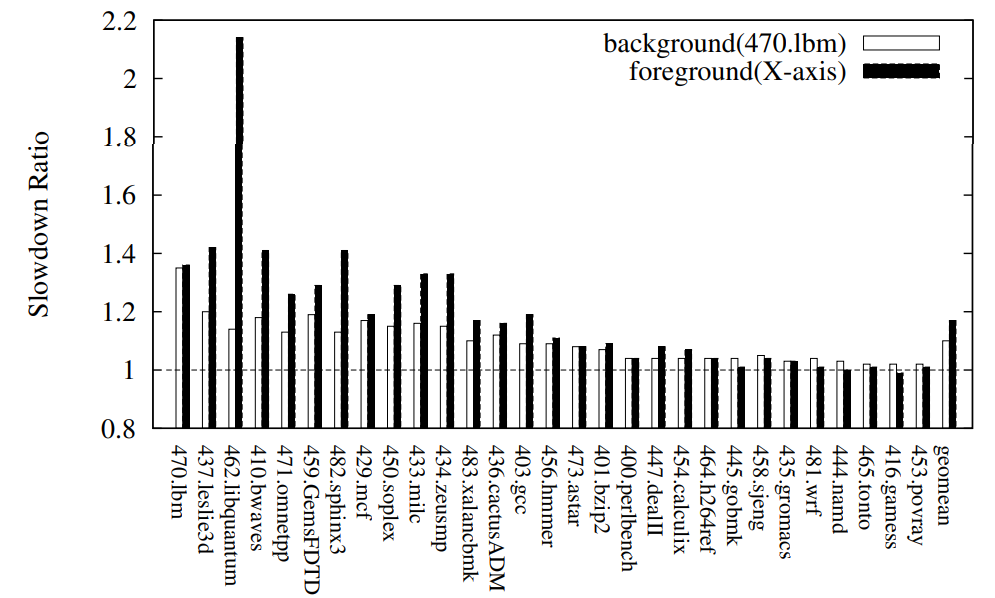
\includegraphics[width=0.80\columnwidth]{memguard.png}
        \caption{IPC slowdown of foreground (X-axis) and background
        task (470.lbm) on a dual-core configuration}
        \label{fig:TraceEnable}
    \end{figure}
\end{frame}

\begin{frame}
    \frametitle{Problems of Shared Memory in Multi-core Systems}
    \begin{itemize}
        \item In embedded systems, task execution time is increasingly more
            dependent on the way that memory resources are allocated among
            cores.
        \item Allocation Schemes used by the allocator does not take into
            account the addresses of the allocated chunks.
        \item Results indicate that memory bandwidth is very different
            compared to CPU bandwidth, in the sense that maximum achievable
            bandwidth is not fixed but highly variable depending on access
            location of each memory request and on the state of DRAM subsystem.
    \end{itemize}
\end{frame}

\begin{frame}
    \frametitle{MemGuard: How its Done}
    \begin{itemize}
        \item Regulate each core request rate.
        \item Programs PMC to generate an interrupt in which it deschedules
            tasks unitl the next hyperperiod.
        \item The rest of their algorithm is focused on bandwidth reuse and
            repurposing for different cores.
    \end{itemize}
\end{frame}

\begin{frame}
    \frametitle{What can we do better using ETM}
    \begin{itemize}
        \item With ETM we are aware of the data address of memory acesses
            \begin{itemize}
                \item Make a more accurate estimation of the DRAM service rate.
                \item Divide DMA and memory accesses.
                \item Make assumption on Virtual Machines making different
                    accesses.
            \end{itemize}
    \end{itemize}
\end{frame}

\begin{frame}
    \frametitle{Hardware Features for Memory Bandwidth Control}
    \begin{itemize}
        \item New hardware features are designed for memory bandwidth control.
        \item Intel Resouce Director Technology and Arm Memory Partitioning
            and Monitoring are the example of such systems.
        \item An research group at INSA de Toulouse states in a poster for new
            candidates (posted 60 days ago) that new task models and scheduling
            algorithms should be defined in response to such hardware.
    \end{itemize}
\end{frame}

\begin{frame}
    \frametitle{Arm Memory System Resource Partitioning and Monitoring (MPAM)
    Extension}
    \begin{itemize}
        \item MPAM extends adds the ability for software to manage resources
            such as:
            \begin{itemize}
                \item Caches
                \item Memory Controllers
            \end{itemize}
        \item Such resource control requires runtime reaction and continuous
            tracking. Also there are requirements due to execptions and
            different security states.
        \item MPAM has following features:
            \begin{itemize}
                \item Memory-system resource partitioning
                \item Memory-system resource usage monitoring
            \end{itemize}
    \end{itemize}
\end{frame}

\begin{frame}
    \begin{figure}
        \centering
        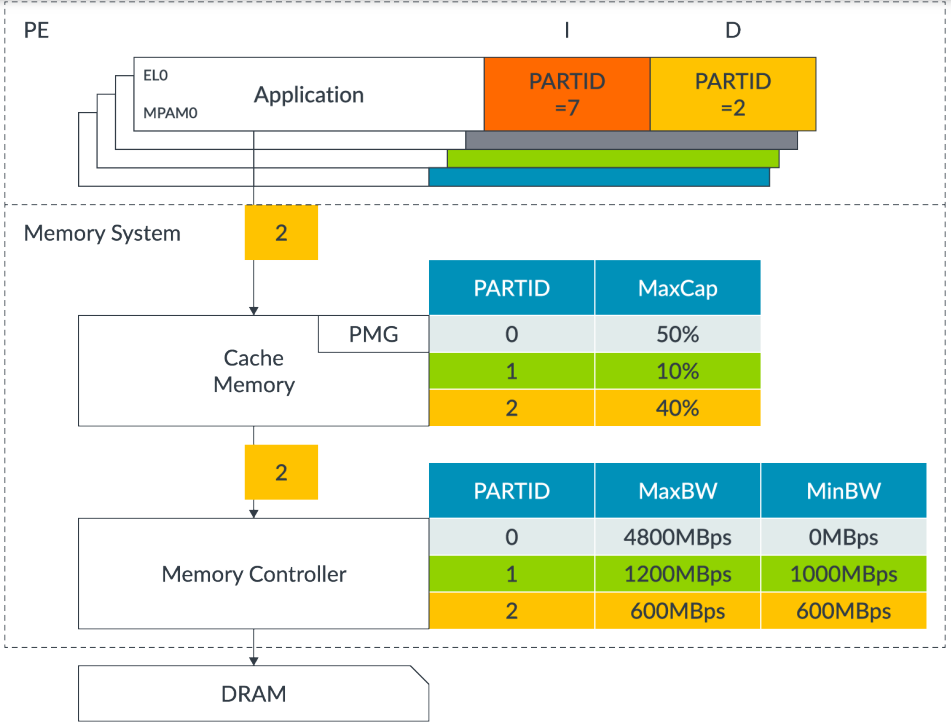
\includegraphics[width=0.80\columnwidth]{mpam.png}
        \caption{Example MPAM Usage}
        \label{fig:MPAM}
    \end{figure}
\end{frame}

\begin{frame}
  \centering \Large
  \emph{Thank You For Your Attention}
\end{frame}

\end{document}
